\chapter{Evaluation}
\label{chap:eval}

In this chapter, we demonstrate the effectiveness of the tokenizer with several
tokenization schemes and on several datasets. In the first section, we study
the accuracy of the tokenizer set up in wildly different manners. In the
second section, we follow up with an analysis of the speed at which it
processes data.

\section{The Accuracy of the System}
\label{sec:eval-acc}

\subsection{Chinese Word Segmentation}
\label{ssec:eval-acc-chinese}

Tokenizing Latin-script languages is not very hard. We can usually get by well
enough by splitting the text at whitespaces and at boundaries between different
classes of symbols. Sometimes, we might want to be more specific and try to
tokenize English contractions as separate words. However, these problems are
quite easy to solve when compared to the task of tokenizing Chinese text. The
absence of any spaces between words forbids the use of any simple heuristic and
linguistically empowered methods must be used.

We took inspiration from the system for Chinese word segmentation presented in
Section~\ref{survey-chinese} \cite{seg-chinese-maxent} which is also based on
maximum entropy models. The basic features used in that system were ported to
our formalism. The biggest difference between the systems is the fact that the
original Chinese tokenizer classified individual characters as being
single-character words or the beginning, middle or ending characters of a
multi-character word. However, the classifier used in our system is binary and
it decides for each character boundary whether it forms a token boundary or
not.

We were able to obtain the same data on which the original tokenizer was
developed, which happen to be the training data for the Second International
Chinese Word Segmentation Bakeoff \cite{web-bakeoff}. The bakeoff was a
competition challenging computational linguists to develop word segmentation
systems for Chinese using the supplied data for training. The provided data
consists of 4 datasets provided by Academia Sinica, City University of Hong
Kong, Peking University and Microsoft Research. Each of these datasets adopts
slightly different tokenization standards and so we train and test our
tokenizer on the datasets individually. Each dataset comes with a training part
and a testing part. We strictly used only the training part when developing our
tokenizer and used the testing part only at the end to evaluate our results.
The only thing we knew about the testing data in advance was its size which
helped us choose a reasonable size for our heldout data.

First off, we split our training data into a development part and a heldout
part. We chose the size of the heldout data to be roughly as big as the testing
data so we could trust our system's performance on it to be representative of
our system's true accuracy. The sizes of the partitioned datasets can be seen
in Table~\ref{tbl:bakeoff-sizes}.

\begin{table}
  \begin{center}
    \begin{tabular}{ | l | r | r | r | }
      \hline
      & \multicolumn{2}{ | c | }{Training data} & Testing data \\ \hline
      & Development data & Heldout data & Testing data \\ \hline
      Academia Sinica & 39686533 & 1057344 & 942571 \\ \hline
      City University & 8283422 & 266247 & 240767 \\ \hline
      Peking University & 7008808 & 719430 & 718331 \\ \hline
      Microsoft Research & 16100177 & 791333 & 766786 \\
      \hline
    \end{tabular}
  \end{center}
  \caption[Bakeoff dataset sizes]
    {The sizes of the individual parts of the bakeoff datasets in bytes.}
  \label{tbl:bakeoff-sizes}
\end{table}

Initially, we set the event cutoff of the maximum entropy trainer to 2 as in
\cite{seg-chinese-maxent}. However, we found out we get a sizable improvement
in the accuracy of the trained tokenizer if we do not cutoff events (i.e. set
the event cutoff to 1). We then experimented with training the tokenizer and
testing it on the heldout data. Depending on how much we constrained training
time, the tokenizer could either be under-trained or over-fitted. The heldout
data served as an independent indicator telling us how close we are to the
ideal balance between a detailed and a general model. Experimentation led us to
restrain the number of training iterations to the values seen in
Table~\ref{tbl:bakeoff-iters} (the considerable size of the Academia Sinica
combined with the absence of the event cutoff forced us to keep the number of
training iterations below 450 lest the training program hit the CPU time
limit and terminate). We can see that the number of iterations spent training
to obtain the optimal model correlates with the size of the dataset (with the
exception of the Academia Sinica dataset, of course), because a larger dataset
usually means more bigrams and unigrams and thus more parameters to estimate.

\begin{table}
  \begin{center}
    \begin{tabular}{ | l | r | }
      \hline
      & Number of iterations \\ \hline
      Academia Sinica & 420 \\ \hline
      City University & 873 \\ \hline
      Peking University & 708 \\ \hline
      Microsoft Research & 1053 \\
      \hline
    \end{tabular}
  \end{center}
  \caption[Number of training iterations for Chinese segmentation]
    {The number of iterations spent training the maximum entropy model on the
    individual datasets.}
  \label{tbl:bakeoff-iters}
\end{table}

After we established the training parameters, we trained the system on the
entire training data and checked its performance on the gold testing data. The
performance of the development system on the heldout data and of the final
system on the testing data can be seen in Tables \ref{tbl:bakeoff-devel} and
\ref{tbl:bakeoff-final}.

\begin{table}
  \begin{center}
    \begin{tabular}{ | l | r | r | r | r | }
      \hline
      & Accuracy & Precision & Recall & F-measure \\ \hline
      Academia Sinica & 97.56\% & 97.89\% & 97.82\% & 97.86\% \\ \hline
      City University & 97.70\% & 98.05\% & 98.11\% & 98.08\% \\ \hline
      Peking University & 97.69\% & 98.29\% & 97.89\% & 98.09\% \\ \hline
      Microsoft Research & 97.67\% & 98.08\% & 98.02\% & 98.05\% \\
      \hline
    \end{tabular}
  \end{center}
  \caption[Development performance of Chinese segmenter]
    {The performance of the system trained on the development data when
     tokenizing the heldout data.}
  \label{tbl:bakeoff-devel}
\end{table}

\begin{table}
  \begin{center}
    \begin{tabular}{ | l | r | r | r | r | }
      \hline
      & Accuracy & Precision & Recall & F-measure \\ \hline
      Academia Sinica & 96.33\% & 96.13\% & 97.73\% & 96.92\% \\ \hline
      City University & 96.87\% & 97.42\% & 97.32\% & 97.37\% \\ \hline
      Peking University & 96.74\% & 97.85\% & 96.68\% & 97.26\% \\ \hline
      Microsoft Research & 97.95\% & 98.33\% & 98.06\% & 98.20\% \\
      \hline
    \end{tabular}
  \end{center}
  \caption[Final performance of Chinese segmenter]
    {The performance of the system trained on the entire training data when
     tokenizing the gold testing data.}
  \label{tbl:bakeoff-final}
\end{table}


We were encouraged to see such performance and out of curiosity proceeded to
score our tokenizer using the same script which scored the contestants in the
bakeoff (Table~\ref{tbl:bakeoff-score}). While our tokenizer does not perform
as well as the original word segmenter by Low, Ng and Guo
\cite{seg-chinese-maxent}, it achieves a median performance compared to the
performance of the other bakeoff submissions. The result is quite pleasing,
given that the all we needed to do was to write the feature definitions into a
few files and toy with some training parameters.

\begin{table}
  \begin{center}
    \begin{tabular}{ | l | r | r | r | r | }
      \hline
      & True Words Recall & Test Words Precision & F-measure \\ \hline
      Academia Sinica & 0.933 & 0.919 & 0.926 \\ \hline
      City University & 0.934 & 0.934 & 0.934 \\ \hline
      Peking University & 0.923 & 0.933 & 0.928 \\ \hline
      Microsoft Research & 0.951 & 0.952 & 0.951 \\
      \hline
    \end{tabular}
  \end{center}
  \caption[Chinese Word Segmentation scores]
    {The scores assigned to our tokenizer by the official scoring script of the
    Second International Chinese Word Segmentation Bakeoff.}
  \label{tbl:bakeoff-score}
\end{table}


\subsection{Tokenization of Czech and English}
\label{ssec:eval-acc-eng}

For evaluating the accuracy of tokenizing Czech and English text, four
different methods were implemented. The Absolute Baseline relies on no other
piece of information than the current decision point and the whitespace
following it to classify boundaries. It is there to show the minimum possible
line every tokenizer should pass. The Simple Tokenizer checks the potential
sentence terminator and checks whether the following word starts with an
upper-case letter. It represents the often too simple approach to tokenization.
The English-only Satz-like \cite{sbd-satz} system uses only part of speech data
about the surrounding tokens to predict a boundary. Finally, the Groomed
Tokenizer is the tokenization scheme used in the original reference
implementation, which has been supplied with lists of abbreviations and lots of
useful regular expressions.

All systems were tested both on a sample of data from CzEng and, in the case of
the English tests, also on the Brown corpus. All datasets were divided into
equally large development, heldout and testing sets to be used as in
Section~\label{ssec:eval-acc-chinese}. As for the part of speech data of the
Satz-like system, lexicons for each part of speech were extracted from the
training section of the Brown corpus for the Brown corpus exercise and from the
entire Brown corpus for the CzEng exercise. The results of the trials can be
seen on Tables~\ref{tbl:czeng-czseg}, \ref{tbl:czeng-cztok},
\ref{tbl:czeng-enseg}, \ref{tbl:czeng-entok}, \ref{tbl:brown-seg} and
\ref{tbl:brown-tok}.

\begin{table}
  \begin{center}
    \begin{tabular}{ | l | c | c | c | c | c | }
      \hline
      CzEng - Czech & \multicolumn{4}{ | c | }{Segmentation} \\ \hline
      & Acc. & Prec. & Rec. & F-m. \\ \hline
      Absolute Baseline & 80.08\% & 72.72\% & 99.06\% & 83.87\% \\ \hline
      Simple Tokenizer & 93.67\% & 92.38\% & 95.79\% & 94.06\% \\ \hline
      Groomed Tokenizer & 95.93\% & 95.26\% & 96.90\% & 96.07\% \\
      \hline
    \end{tabular}
  \end{center}
  \caption[Segmentation performance on Czech]
    {The sentence boundary disambiguation performance of the various methods
     for tokenizing Czech on the CzEng sample.}
  \label{tbl:czeng-czseg}
\end{table}

\begin{table}
  \begin{center}
    \begin{tabular}{ | l | c | c | c | c | c | }
      \hline
      CzEng - Czech & \multicolumn{4}{ | c | }{Tokenization} \\ \hline
      & Acc. & Prec. & Rec. & F-m. \\ \hline
      Absolute Baseline & 99.29\% & 99.29\% & 100.00\% & 99.64\% \\ \hline
      Simple Tokenizer & 99.26\% & 99.35\% & 99.92\% & 99.63\% \\ \hline
      Groomed Tokenizer & 99.36\% & 99.39\% & 99.97\% & 99.68\% \\
      \hline
    \end{tabular}
  \end{center}
  \caption[Tokenization performance on Czech]
    {The token boundary disambiguation performance of the various methods for
     tokenizing Czech on the CzEng sample.}
  \label{tbl:czeng-cztok}
\end{table}

\begin{table}
  \begin{center}
    \begin{tabular}{ | l | c | c | c | c | c | }
      \hline
      CzEng - English & \multicolumn{4}{ | c | }{Segmentation} \\ \hline
      & Acc. & Prec. & Rec. & F-m. \\ \hline
      Absolute Baseline & 81.27\% & 67.50\% & 99.91\% & 80.57\% \\ \hline
      Simple Tokenizer & 95.21\% & 91.38\% & 96.81\% & 94.01\% \\ \hline
      Satz-like System & 94.87\% & 92.42\% & 94.57\% & 93.48\% \\ \hline
      Groomed Tokenizer & 97.08\% & 95.66\% & 96.90\% & 96.27\% \\
      \hline
    \end{tabular}
  \end{center}
  \caption[Segmentation performance on English CzEng]
    {The sentence boundary disambiguation performance of the various methods
     for tokenizing English on the CzEng sample.}
  \label{tbl:czeng-enseg}
\end{table}

\begin{table}
  \begin{center}
    \begin{tabular}{ | l | c | c | c | c | c | }
      \hline
      CzEng - English & \multicolumn{4}{ | c | }{Tokenization} \\ \hline
      & Acc. & Prec. & Rec. & F-m. \\ \hline
      Absolute Baseline & 95.31\% & 95.31 & 100.00\% & 97.60\% \\ \hline
      Simple Tokenizer & 95.27\% & 95.31\% & 99.95\% & 97.58\% \\ \hline
      Satz-like System & 96.84\% & 96.79\% & 100.00\% & 98.37\% \\ \hline
      Groomed Tokenizer & 95.99\% & 95.99\% & 99.98\% & 97.94\% \\
      \hline
    \end{tabular}
  \end{center}
  \caption[Tokenization performance on English CzEng]
    {The token boundary disambiguation performance of the various methods for
     tokenizing English on the CzEng sample.}
  \label{tbl:czeng-entok}
\end{table}

\begin{table}
  \begin{center}
    \begin{tabular}{ | l | c | c | c | c | c | }
      \hline
      Brown & \multicolumn{4}{ | c | }{Segmentation} \\ \hline
      & Acc. & Prec. & Rec. & F-m. \\ \hline
      Absolute Baseline & 78.49\% & 62.83\% & 99.61\% & 77.06\% \\ \hline
      Simple Tokenizer & 96.47\% & 93.26\% & 97.30\% & 95.24\% \\ \hline
      Satz-like System & 99.31\% & 99.58\% & 98.52\% & 99.05\% \\ \hline
      Groomed Tokenizer & 99.31\% & 99.30\% & 98.80\% & 99.05\% \\
      \hline
    \end{tabular}
  \end{center}
  \caption[Segmentation performance on Brown]
    {The sentence boundary disambiguation performance of the various methods
     for tokenizing English on the Brown corpus.}
  \label{tbl:brown-seg}
\end{table}

\begin{table}
  \begin{center}
    \begin{tabular}{ | l | c | c | c | c | c | }
      \hline
      Brown & \multicolumn{4}{ | c | }{Tokenization} \\ \hline
      & Acc. & Prec. & Rec. & F-m. \\ \hline
      Absolute Baseline & 82.71\% & 85.16\% & 88.74\% & 86.91\% \\ \hline
      Simple Tokenizer & 93.63\% & 94.12\% & 96.16\% & 95.13\% \\ \hline
      Satz-like System & 99.64\% & 99.62\% & 99.82\% & 99.72\% \\ \hline
      Groomed Tokenizer & 99.73\% & 99.72\% & 99.86\% & 99.79\% \\
      \hline
    \end{tabular}
  \end{center}
  \caption[Tokenization performance on Brown]
    {The token boundary disambiguation performance of the various methods for
     tokenizing English on the Brown corpus.}
  \label{tbl:brown-tok}
\end{table}

While segmenting text from the CzEng dataset proves to be more difficult for
all but the Baseline tokenizer, the Satz-like system's segmentation performance
suffers the most. This was not unexpected as the Satz-like tokenizer relies on
a lexicon of part of speech tags extracted from parts of the Brown corpus. When
the tokenizer was evaluated on the Brown corpus, the lexicon was induced from
the training and heldout datasets. This gave the tokenizer's lexicon a 99.41\%
coverage on the training dataset and a 99.44\% coverage on the heldout dataset
(the coverage is not 100\% as some of the words containing dashes or
apostrophes were broken into separate rough tokens); the coverage on the
testing dataset was 95.75\%. On the other hand, when the tokenizer was
evaluated on the CzEng dataset, the coverage on the training, heldout and
testing datasets was 95.80\%, 95.95\% and 95.66\% respectively. This gives the
Satz-like tokenizer an advantage over the Brown corpus as the training data is
used to its full potential.

The Simple tokenizer demonstrates a pretty high recall on sentence boundary
detection. This can be attributed to the fact that its decisions are governed
only by the potential sentence boundary and the case of the following word.
Since mostly every sentence will start with a capital letter, we can expect the
Simple tokenizer to notice most of them. The Simple tokenizer can however be
easily misled by multi-part abbreviations and initials in names (e.g.
``U.S.A.'', ``M. Smith''). This explains why its precision is noticeably
lower than its recall.

\section{The Speed of the System}
\label{sec:eval-spd}

\subsection{Parallel Processing}
\label{ssec:eval-spd-parallel}

One of the most important aspects of the tokenizer which drove the design was
parallel processing. In Chapter~\ref{chap:impl}, we have seen how it encouraged
us to divide the tokenizer's duties to several autonomous subsystems. This
design enabled us to perform all the tasks in the pipeline in parallel using
the \class{pipeline} class from the Threading Building Blocks library
\cite{web-tbb}. To measure the impact this design choice made on performance,
we ran the tokenizer on the entire Brown corpus while restricting the maximum
number of pipeline stages allowed to run at the same time. The results are
plotted in Figure \ref{fig:plot-work-units}. The Baseline and Groomed
tokenizers speed up by 17\%--19\%, while the Simple and Satz-like tokenizers
gain a speedup of 31\%.

\begin{figure}
  \begin{center}
    % GNUPLOT: LaTeX picture with Postscript
\begingroup
  \makeatletter
  \providecommand\color[2][]{%
    \GenericError{(gnuplot) \space\space\space\@spaces}{%
      Package color not loaded in conjunction with
      terminal option `colourtext'%
    }{See the gnuplot documentation for explanation.%
    }{Either use 'blacktext' in gnuplot or load the package
      color.sty in LaTeX.}%
    \renewcommand\color[2][]{}%
  }%
  \providecommand\includegraphics[2][]{%
    \GenericError{(gnuplot) \space\space\space\@spaces}{%
      Package graphicx or graphics not loaded%
    }{See the gnuplot documentation for explanation.%
    }{The gnuplot epslatex terminal needs graphicx.sty or graphics.sty.}%
    \renewcommand\includegraphics[2][]{}%
  }%
  \providecommand\rotatebox[2]{#2}%
  \@ifundefined{ifGPcolor}{%
    \newif\ifGPcolor
    \GPcolorfalse
  }{}%
  \@ifundefined{ifGPblacktext}{%
    \newif\ifGPblacktext
    \GPblacktexttrue
  }{}%
  % define a \g@addto@macro without @ in the name:
  \let\gplgaddtomacro\g@addto@macro
  % define empty templates for all commands taking text:
  \gdef\gplbacktext{}%
  \gdef\gplfronttext{}%
  \makeatother
  \ifGPblacktext
    % no textcolor at all
    \def\colorrgb#1{}%
    \def\colorgray#1{}%
  \else
    % gray or color?
    \ifGPcolor
      \def\colorrgb#1{\color[rgb]{#1}}%
      \def\colorgray#1{\color[gray]{#1}}%
      \expandafter\def\csname LTw\endcsname{\color{white}}%
      \expandafter\def\csname LTb\endcsname{\color{black}}%
      \expandafter\def\csname LTa\endcsname{\color{black}}%
      \expandafter\def\csname LT0\endcsname{\color[rgb]{1,0,0}}%
      \expandafter\def\csname LT1\endcsname{\color[rgb]{0,1,0}}%
      \expandafter\def\csname LT2\endcsname{\color[rgb]{0,0,1}}%
      \expandafter\def\csname LT3\endcsname{\color[rgb]{1,0,1}}%
      \expandafter\def\csname LT4\endcsname{\color[rgb]{0,1,1}}%
      \expandafter\def\csname LT5\endcsname{\color[rgb]{1,1,0}}%
      \expandafter\def\csname LT6\endcsname{\color[rgb]{0,0,0}}%
      \expandafter\def\csname LT7\endcsname{\color[rgb]{1,0.3,0}}%
      \expandafter\def\csname LT8\endcsname{\color[rgb]{0.5,0.5,0.5}}%
    \else
      % gray
      \def\colorrgb#1{\color{black}}%
      \def\colorgray#1{\color[gray]{#1}}%
      \expandafter\def\csname LTw\endcsname{\color{white}}%
      \expandafter\def\csname LTb\endcsname{\color{black}}%
      \expandafter\def\csname LTa\endcsname{\color{black}}%
      \expandafter\def\csname LT0\endcsname{\color{black}}%
      \expandafter\def\csname LT1\endcsname{\color{black}}%
      \expandafter\def\csname LT2\endcsname{\color{black}}%
      \expandafter\def\csname LT3\endcsname{\color{black}}%
      \expandafter\def\csname LT4\endcsname{\color{black}}%
      \expandafter\def\csname LT5\endcsname{\color{black}}%
      \expandafter\def\csname LT6\endcsname{\color{black}}%
      \expandafter\def\csname LT7\endcsname{\color{black}}%
      \expandafter\def\csname LT8\endcsname{\color{black}}%
    \fi
  \fi
  \setlength{\unitlength}{0.0500bp}%
  \begin{picture}(7200.00,5040.00)%
    \gplgaddtomacro\gplbacktext{%
      \csname LTb\endcsname%
      \put(946,704){\makebox(0,0)[r]{\strut{} 0}}%
      \put(946,1383){\makebox(0,0)[r]{\strut{} 5}}%
      \put(946,2061){\makebox(0,0)[r]{\strut{} 10}}%
      \put(946,2740){\makebox(0,0)[r]{\strut{} 15}}%
      \put(946,3418){\makebox(0,0)[r]{\strut{} 20}}%
      \put(946,4097){\makebox(0,0)[r]{\strut{} 25}}%
      \put(946,4775){\makebox(0,0)[r]{\strut{} 30}}%
      \put(1078,484){\makebox(0,0){\strut{} 1}}%
      \put(1721,484){\makebox(0,0){\strut{} 2}}%
      \put(2365,484){\makebox(0,0){\strut{} 3}}%
      \put(3008,484){\makebox(0,0){\strut{} 4}}%
      \put(3652,484){\makebox(0,0){\strut{} 5}}%
      \put(4295,484){\makebox(0,0){\strut{} 6}}%
      \put(4939,484){\makebox(0,0){\strut{} 7}}%
      \put(5582,484){\makebox(0,0){\strut{} 8}}%
      \put(6226,484){\makebox(0,0){\strut{} 9}}%
      \put(6869,484){\makebox(0,0){\strut{} 10}}%
      \put(308,2739){\rotatebox{-270}{\makebox(0,0){\strut{}Seconds spent tokenizing the Brown corpus}}}%
      \put(3973,154){\makebox(0,0){\strut{}Maximum number of simultaneous work units}}%
    }%
    \gplgaddtomacro\gplfronttext{%
      \csname LTb\endcsname%
      \put(5882,4602){\makebox(0,0)[r]{\strut{}Groomed Tokenizer}}%
      \csname LTb\endcsname%
      \put(5882,4382){\makebox(0,0)[r]{\strut{}Satz-like Tokenizer}}%
      \csname LTb\endcsname%
      \put(5882,4162){\makebox(0,0)[r]{\strut{}Simple Tokenizer}}%
      \csname LTb\endcsname%
      \put(5882,3942){\makebox(0,0)[r]{\strut{}Baseline Tokenizer}}%
    }%
    \gplbacktext
    \put(0,0){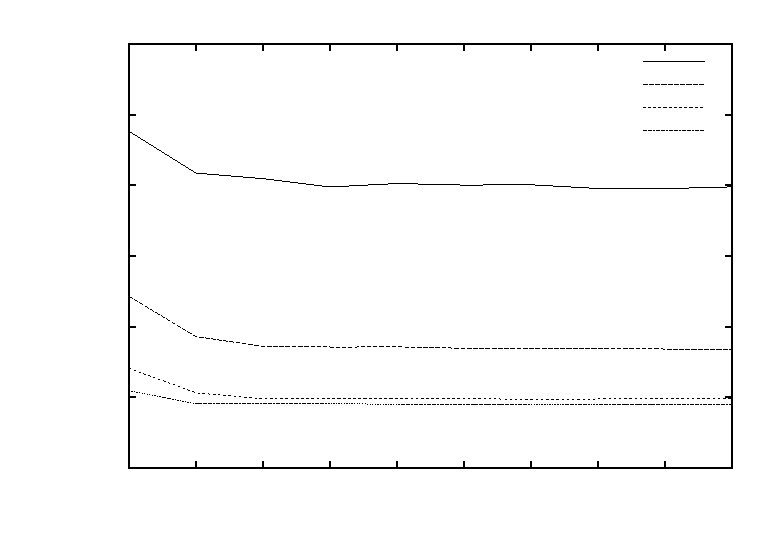
\includegraphics{img/work-units}}%
    \gplfronttext
  \end{picture}%
\endgroup

    \caption{The effect of maximum simultaneous work units on the performance of
             the tokenizer. The plotted spent time is a median of 10 trials.}
    \label{fig:plot-work-units}
  \end{center}
\end{figure}

To investigate the reason why the different tokenization schemes gain a
different speedup and where we should optimize further to improve the
processing time, we measure the workload of the different pipeline stages. We
restrict the maximum number of simultaneous work units in the pipeline to 1, to
ensure that only one can use the CPU at a time. In each of the stages we
measured the total time spent processing the stream of data. The averaged
results can be seen in Table~\ref{tbl:bottlenecks}.

\begin{table}
  \begin{center}
    \begin{tabular}{ | l | r | r | r | r | r | }
      \hline
      & Baseline & Simple & Satz-like & Groomed \\ \hline
      RoughTokenizer & 3.056 & 3.056 & 3.086 & 3.185 \\ \hline
      FeatureExtractor & 0.276 & 0.671 & 2.492 & 5.128 \\ \hline
      Classifier & 1.113 & 2.188 & 5.118 & 14.217 \\ \hline
      OutputFormatter & 0.722 & 0.701 & 0.713 & 0.712 \\
      \hline
    \end{tabular}
  \end{center}
  \caption[Time spent in individual pipeline elements]
    {Time (in seconds) spent in the various pipeline stages when tokenizing the
    Brown corpus. In order to measure these values, the pipeline has been set
    up to run only one stage at a time. The tabled time is an average of 10
    trials.}
  \label{tbl:bottlenecks}
\end{table}

From the data, we can see that the workload is more balanced in the Simple and
Satz-like tokenizers, while in the Baseline and Groomed tokenizers, the
RoughTokenizer, resp. the Classifier, spend almost twice the time the other
stages do. This means that when using the Baseline or Groomed tokenizer, one
thread will be working in the RoughTokenizer, resp. the Classifier, leaving the
other threads very little work to do, which leads to only a small speedup from
the original scenario with one thread.

We can also see that the complexity of rough tokenization and output processing
is the same with all the tokenization schemes, which was to be expected as
there are next to no differences in these stages between the contesting
tokenizers. The FeatureExtractor's workload scales with the number of regular
expression properties and list properties as expected (the data also shows that
the multiple list properties used for the part of speech lexicon in the
Satz-like tokenizer are faster to check than the individual regular expressions
used in the Groomed tokenizer).

The most important fact we can glean from the results, however, is that in the
more complex tokenizers, the Classifier is the bottleneck. The Classifier is
the subsystem responsible for checking the context surrounding each decision
point, producing a list of strings describing the features of the rough tokens
in the context and consulting the maximum entropy model for a disambiguation.

\begin{table}
  \begin{center}
    \begin{tabular}{ | l | c | c | c | c | c | }
      \hline
      & Baseline & Simple & Satz-like & Groomed \\ \hline
      Width of context & 1 & 2 & 7 & 17 \\ \hline
      Number of user-defined properties & 0 & 1 & 37 & 32 \\ \hline
      Number of possible features per decision & 6 & 13 & 311 & 673 \\ \hline
      Average number of features per decision & 1.53 & 3.98 & 21.04 & 75.38 \\
      \hline
    \end{tabular}
  \end{center}
  \caption[Computational complexity of the Classifier stage]
    {The factors which define the computational complexity of the Classifier
    stage. The average number of features per decision was measured on the
    Brown corpus.}
  \label{tbl:classifier-load-factors}
\end{table}

The distinguishing factors which define the computational complexity of the
Classifier are listed in Table~\ref{tbl:classifier-load-factors}. The
Classifier iterates over the rough tokens in the context. Each rough token is
checked for the mandatory properties (whitespace between tokens, presence of
decision points) and strings representing the features are created. The rough
tokens at specific offsets are also checked for the user-defined properties and
strings describing these features are generated as well. This vector of
features is then deciphered by the maximum entropy toolkit. Each feature name
is mapped to a factor and the factors are added up for each individual outcome.
The outcome with the highest probability is then selected.

The amount of work needed to handle the built-in mandatory probabilities is
linear with respect to the width of the context.

The rest of the time is spent checking for the user-defined properties and
generating feature strings (a string containing the offset, name and value of a
feature). Assuming the names of user-defined properties are bound by some
constant, the worst case time spent doing this is linear to the product of the
context's width and the number of user-defined properties. However, at some of
the offsets in the context, some of the properties might not be requested by
the user or might simply not hold for the rough token in question. We let the
tokenizers log the decision points and the features describing them and
measured how much feature strings per decision are actually generated and
processed by the maximum entropy library (the values are listed in Table
\ref{classifier-load-factors}). This factor is most indicative of the
workload of the Classifier.

As the Classifier has been identified as a bottleneck of the pipeline, any
attempts at optimizing the performance of the tokenizer should be performed
there. The amount of time spent in the maximum entropy library is 15\%--23\% of
the entire time spent in the Classifier. Improving the string manipulation and
feature representation thus seem as sensible places to look at. In the case of
the Groomed tokenizer, more speed could be gained by culling the number of
features or narrowing the context.

\subsection{Initialization Costs}
\label{ssec:eval-spd-init}

A necessary part of processing data with the tokenizer is the execution and
initialization of the tokenizer itself. We were interested how long the
initialization takes in comparison to the processing of input. We measured the
time spent in both these stages and listed our measurements in Table
\ref{tbl:timeline}.

\begin{table}
  \begin{center}
    \begin{tabular}{ | l | r | r | r | r | r | }
      \hline
      & Baseline & Simple & Satz-like & Groomed \\ \hline
      Initialization & 0.002 & 0.027 & 0.303 & 0.110 \\ \hline
      Processing & 4.473 & 4.856 & 8.117 & 19.591 \\ \hline
      Total & 4.475 & 4.883 & 8.420 & 19.701 \\
      \hline
    \end{tabular}
  \end{center}
  \caption[Time spent in individual initialization steps]
    {Time (in seconds) spent tokenizing the Brown corpus using the 4
    tokenization schemes presented. Initialization is the time spent before the
    pipeline is run. The tabled time is an average of 10 trials.}
  \label{tbl:timeline}
\end{table}

It can be seen that when processing large quantities of data, the
initialization costs are negligible. However, it is quite probable that the
tokenizer will be used to process smaller files. For example, the entire Brown
corpus has 6MB of data, but is distributed as a set of files about 11KB small.
To express the cost of initialization in more useful terms, we found the volume
of data that the tokenizer can process within the amount of time spent to
initialize it (Table~\ref{tbl:init-sizes}). The data shows that when using the
Simple or the Groomed tokenizer, it would take four times as long to process
the Brown corpus if we were to initialize the tokenizer before processing each
file. When using the Satz-like tokenizer or any other tokenization scheme based
on large lexicons, the initialization costs are even bigger.

\begin{table}
  \begin{center}
    \begin{tabular}{ | l | c | c | c | c | c | }
      \hline
      & Baseline & Simple & Satz-like & Groomed \\ \hline
      Size of data & 530 & 36500 & 269000 & 35500 \\
      \hline
    \end{tabular}
  \end{center}
  \caption[Time spent initializing expressed as time spent processing data]
    {Volumes of data (in bytes) which take the same time to process using a
    given tokenization scheme as it takes to initialize the tokenization
    scheme.}
  \label{tbl:init-sizes}
\end{table}

The expected cost in initialization time is mitigated by the ability to run
the tokenizer on batches of files. The tokenizer can look for files to be
processed in lists of file paths stored in files or passed through the standard
input. The results are written to files whose path is found by applying a
user-specified regular expression replacement string on the original file's
path.

All the tokenization schemes presented in this chapter were trained and
tested using this way of execution. If large volumes of small files are to be
processed using the tokenizer, these batch facilities are essential as they
make the daunting cost of initialization marginal (as in Table
\ref{tbl:timeline}).
